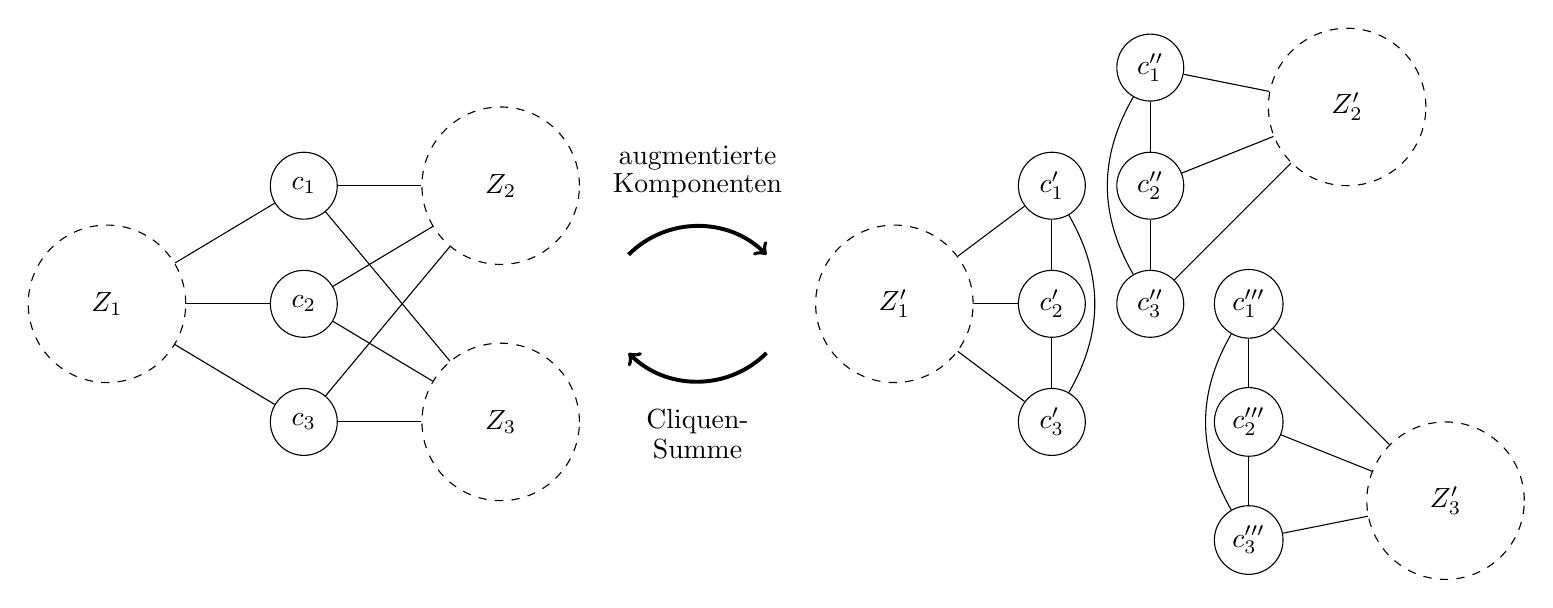
\begin{tikzpicture}

\node [circle, minimum height=0.85cm, draw] (v1) at (0,0.5) {$c_1$};
\node [circle, minimum height=0.85cm, draw] (v5) at (0,-1) {$c_2$};
\node [circle, minimum height=0.85cm, draw] (v6) at (0,-2.5) {$c_3$};
\node [circle, minimum height=2cm, draw, dashed] (v2) at (-2.5,-1) {$Z_1$};
\node [circle, minimum height=2cm, draw, dashed] (v3) at (2.5,0.5) {$Z_2$};
\node [circle, minimum height=2cm, draw, dashed] (v4) at (2.5,-2.5) {$Z_3$};
\draw  (v1) edge (v2);
\draw  (v1) edge (v3);
\draw  (v1) edge (v4);
\draw  (v5) edge (v2);
\draw  (v5) edge (v3);
\draw  (v5) edge (v4);
\draw  (v6) edge (v2);
\draw  (v6) edge (v3);
\draw  (v6) edge (v4);


\node [circle, minimum height=2cm, draw, dashed] (v7) at (7.5,-1) {$Z_1'$};
\node [circle, minimum height=0.85cm, draw] (v9) at (9.5,-1) {$c_2'$};
\node [circle, minimum height=0.85cm, draw] (v8) at (9.5,0.5) {$c_1'$};
\node [circle, minimum height=0.85cm, draw] (v10) at (9.5,-2.5) {$c_3'$};
\draw  (v7) edge (v8);
\draw  (v7) edge (v9);
\draw  (v7) edge (v10);
\draw  (v8) edge (v9);
\draw  (v9) edge (v10);
\draw [bend right] (v10) edge (v8);

\node [circle, minimum height=0.85cm, draw] (v12) at (10.75,2) {$c_1''$};
\node [circle, minimum height=0.85cm, draw] (v13) at (10.75,0.5) {$c_2''$};
\node [circle, minimum height=0.85cm, draw] (v14) at (10.75,-1) {$c_3''$};
\node [circle, minimum height=2cm, draw, dashed] (v11) at (13.25,1.5) {$Z_2'$};
\draw  (v11) edge (v12);
\draw  (v11) edge (v13);
\draw  (v11) edge (v14);
\draw  (v12) edge (v13);
\draw  (v13) edge (v14);
\draw [bend right] (v12) edge (v14);

\node [circle, minimum height=0.85cm, draw] (v16) at (12,-1) {$c_1'''$};
\node [circle, minimum height=0.85cm, draw] (v17) at (12,-2.5) {$c_2'''$};
\node [circle, minimum height=0.85cm, draw] (v18) at (12,-4) {$c_3'''$};
\node [circle, minimum height=2cm, draw, dashed] (v15) at (14.5,-3.5) {$Z_3'$};
\draw  (v15) edge (v16);
\draw  (v15) edge (v17);
\draw  (v15) edge (v18);
\draw  (v16) edge (v17);
\draw  (v17) edge (v18);
\draw [bend right] (v16) edge (v18);


\node [] (v19) at (4,-0.5) {};
\node [] (v20) at (6,-0.5) {};
\draw [->, bend left=45, line width=0.05cm] (v19) edge (v20);

\node (v21) at (6,-1.5) {};
\node (v22) at (4,-1.5) {};
\draw [->, bend left=45, line width=0.05cm] (v21) edge (v22);

\node at (5,0.85) {augmentierte};
\node at (5,0.5) {Komponenten};
\node at (5,-2.5) {Cliquen-};
\node at (5,-2.85) {Summe};
\end{tikzpicture}